\documentclass[11pt]{article}

\newcommand{\Moser}{M{\"o}ser}

\usepackage{algorithm2e}
\usepackage{amssymb}
\usepackage[english]{babel}
\usepackage{changepage}
\usepackage{cite}
\usepackage{float}
\usepackage[margin=1.5in]{geometry}
\usepackage{graphicx}
\usepackage[utf8]{inputenc}
\usepackage{listings}
\usepackage{lmodern}
\usepackage{setspace}
\usepackage{supertabular}
\usepackage{tabularx}
\usepackage{tikz}
\usepackage{url}

\usepackage[T1]{fontenc}

\lstset{
    basicstyle=\small,
    showspaces=false,
    showstringspaces=false,
    tabsize=2,
    title=\lstname,
}

\graphicspath{{figures}}

\onehalfspacing

\begin{document}
\thispagestyle{empty}
\begin{center}
    \begin{Large}
        \emph{Master's Thesis} \\
        Department of Computer Science \\
        Rochester Institute of Techology \\
    \end{Large}
    \vspace{4em}
    {\huge Anonymity Analysis of Cryptocurrencies} \\
    \vspace{3em}
    {\LARGE Liam Morris} \\
    {\tt lcm1115@rit.edu} \\
    \vspace{3em}
    \begin{adjustwidth}{.5in}{.5in}
        Chair: Professor Stanis{\l}aw Radziszowski \hfill {\tt spr@cs.rit.edu} \\
        \vspace{2em}
        \hrulefill \\
        \vspace{3em}
        Reader: Professor Warren Carithers \hfill {\tt wrc@cs.rit.edu} \\
        \vspace{2em}
        \hrulefill \\
        \vspace{3em} Observer: Professor Bo Yuan \hfill {\tt bo.yuan@rit.edu} \\
        \vspace{2em}
        \hrulefill
    \end{adjustwidth}
    \vspace{2em} Rochester, NY 14623 USA \\
    \vspace{2em}
    January 5, 2014
\end{center}
\pagebreak
\thispagestyle{empty}
\begin{abstract}
    Cash in the real world allows for parties to exchange currency without the need to go through some sort of central
    authority. One person, Alice, can simply hand cash over to another person, Bob. In this transaction the only two
    people that have knowledge of this exchange are Alice and Bob. Until recently there was no electronic equivalent to
    this exchange. In 1982 David Chaum proposed a system of anonymous electronic cash based on blind signatures, and in
    1990 founded DigiCash as an electronic cash company. There were a few banks that implemented electronic cash
    systems, but these banks and DigiCash ultimately went bankrupt in 1997 and 1998 despite the enthusiasm surrounding
    anonymous electronic cash.  Between 1998 and 2008 there were no successful implementations of electronic cash that
    offer a decentralized, anonymous, and untraceable system.

    In 2008 a paper was published by Satoshi Nakamoto on the cryptocurrency known as Bitcoin.  A cryptocurrency is a form of
    electronic cash backed by mathematical and cryptographic constructs, unlike traditional currency which was historically
    backed by gold or silver. Cryptocurrencies have seen rising popularity in recent years due to their decentralized,
    distributed, peer-to-peer protocols. Part of this rising popularity is also attributable to the supposed anonymity of
    these protocols; however, due to the public transaction history required for these protocols and the fact that
    transactions are pseudonymous and not purely anonymous, this supposed anonymity does not exist. While the systems may
    achieve the goal of decentralized currency it does not achieve the goal of untraceability. In this thesis we analyze the
    technical implementations of Bitcoin and other cryptocurrencies to determine the level of anonymity provided by these
    protocols. We also analyze proposed improvements for their feasibility. 
\end{abstract}
\clearpage
\pagenumbering{arabic}
\tableofcontents
\listoffigures
\pagebreak
\section{Problem Statement}
Cash in the real world allows for parties to exchange currency without the need to go through some sort of central
authority. One person, Alice, can simply hand cash over to another person, Bob. In this transaction the only two people
that have knowledge of this exchange are Alice and Bob. Until recently there was no electronic equivalent to this
exchange. In 1982 David Chaum proposed a system of anonymous electronic cash based on blind signatures~\cite{chaum83},
and in 1990 founded DigiCash as an electronic cash company. There were a few banks that implemented electronic cash
systems, but these banks and DigiCash ultimately went bankrupt in 1997 and 1998 despite the enthusiasm surrounding
anonymous electronic cash.  Between 1998 and 2008 there were no successful implementations of electronic cash that offer
a decentralized, anonymous, and untraceable system.

In 2008 a paper was published by Satoshi Nakamoto on the cryptocurrency known as Bitcoin~\cite{nakamoto08}.  A
cryptocurrency is a form of electronic cash backed by mathematical and cryptographic constructs, unlike traditional
currency which was historically backed by gold or silver. The Bitcoin protocol uses the SHA-256 algorithm as part of its
cryptographic foundation, while many others such as Litecoin are founded on the scrypt key derivation scheme proposed by
Colin Percival in 2009~\cite{percival09}.  Cryptocurrencies have seen rising popularity in recent years due to their
decentralized, distributed, peer-to-peer protocols. Part of this rising popularity is also attributable to the supposed
anonymity of these protocols; however, due to the public transaction history required for these protocols and the fact
that transactions are pseudonymous and not purely anonymous, this supposed anonymity does not exist. While the systems
may achieve the goal of decentralized currency, they do not achieve the goal of untraceability. There have been
proposals in recent years such as the Zerocoin~\cite{miers13} and Mixcoin~\cite{bonneau14} protocols to remove all
traceability from the Bitcoin protocol. In this thesis we analyze the technical implementations of the Bitcoin and
Litecoin protocols to determine the level of anonymity and traceability provided by these protocols. We also analyze
proposed improvements, such as Zerocoin and Mixcoin, to determine their feasibility and possible optimizations that can
be made.

\section{Cryptographic Tools}

\subsection{Hash Functions} A hash function is an algorithm that processes variable length inputs to produce a fixed
length digest. Hash functions are important for cryptocurrency protocols as they provide the basis on which their
proof-of-work schemes are constructed.

Cryptographic hash functions are designed in such a way that they are non-invertible. In other words, if we have
computed a digest of some message we should not be able to easily deduce the message from the digest. For a hash
function to be secure, the following criteria must uphold~\cite{rogaway04}:

\begin{description}
    \item[Preimage Resistant] Given a digest $H(M)$, it must be computationally difficult to determine
        $M$.
    \item[Second Preimage Resistant] Given a message $M_1$, it must be computationally difficult to determine
        a second message $M_2$ such that $H(M_1) = H(M_2)$. 
    \item[Collision Resistant] It must be computationally
        difficult to construct two messages $M_1$ and $M_2$ such that $H(M_1) = H(M_2)$.
\end{description}

Hash functions are frequently used to uniquely identify large messages so that they may be efficiently signed. In the
case of cryptocurrency protocols this typically takes on the form of hashing an entire transaction so that just the
digest may be signed by a user. In a transaction between Alice and Bob, Alice could construct a transaction and sign
every parameter with her private key individually, which must then be verified with her public key individually.  This
amount of computation is wasteful on both ends, but Alice can use hashing to reduce the amount of computation required.
She can construct the transaction as before, but instead of signing every component she can hash the transaction
parameters together and then sign the resulting digest. On the other end only verification of the signed digest is
required.

\subsubsection{Secure Hash Algorithm}
The Secure Hash Algorithm (SHA) is a family of algorithms published by the National Institute of Standards and
Technology (NIST). In order for an algorithm to be included in the SHA family it must be selected as a winner by NIST in
one of its hash function competitions.

Bitcoin and Litecoin both use the SHA-256 variant of the SHA-2 algorithm as part of their proof-of-work
scheme\footnote{Litecoin uses {\sc scrypt} for its proof-of-work scheme, but {\sc scrypt} performs two {\sc SHA-256}
hashes as part of the algorithm.}. The SHA-256 function hashes a message $M$ in the following manner~\cite{nist}:

\begin{enumerate}
    \item Pad $M$ so that it is on a 512-bit boundary.
    \item Divide $M$ into 512-bit blocks $M_1, M_2, \ldots, M_n$.
    \item Compute $H(M_i) = H(M_i) \boxplus H(M_{i - 1})$ for $i = 1$ to $n$, where $H(M)$ is defined
        as the hashing operation on one block, $H(M_0)$ is a fixed initial hash value, and $\boxplus$ is defined as
        integer addition modulo $2^{32}$.
    \item Output $H(M_n)$ as resulting hash.
\end{enumerate}

Currently NIST states that the SHA-2 algorithm is still cryptographically
secure\footnote{\url{http://csrc.nist.gov/groups/ST/hash/policy.html} -- Accessed 4-1-2014}. If a vulnerability is found
then there is the potential for attacks on cryptocurrencies, so it is worth examining the more recent SHA-3 Keccak
family. The SHA-3 algorithm is not necessarily more secure than SHA-2; however, it is very different structurally so it
is unlikely that both SHA-2 and SHA-3 would be vulnerable to a single attack.

The SHA-3 algorithm uses a sponge construction, which processes variable length input to produce a corresponding
infinite length output. If a fixed length output is desired the output of a sponge function is truncated to the
specified length. Given a permutation $f$, a sponge function operates in the following manner~\cite{bertoni07}:
\vspace{1em}\\
\begin{algorithm}[H]
    \KwIn{$P$ = list of input characters, $n$ = desired hash length}
    \KwOut{$h_0, h_1, \ldots$ = output characters}
    $S \gets \emptyset$ \\
    \For{$p \in P$}{ $S \gets f(S \oplus p)$ }
    \For{$i = 1, 2, \ldots, n$}{ {\sc Output($S$)} \\
    $S \gets f(S)$ }
\end{algorithm}

The specific details for SHA-3 are as follows\cite{sha3}:
\begin{itemize}
    \item \emph{w} - size in bits of state words
    \item \emph{a} - overall state which consists of 5x5 ``sheets'' of \emph{w}-bit words
    \item $\Theta$ - parity of 5-bit columns to be XORed into other columns
    \item $\rho$ - bitwise rotation operation, where each word is rotated by a triangular number
    \item $\pi$ - permutation of state, $a[j][2i+3j] \leftarrow a[i][j]$
    \item $\chi$ - bitwise combination operation of rows
    \item $\iota$ - XOR operation, XOR round constant into single word of state
\end{itemize}

Each round of SHA-3 uses the following function (\emph{Round}, where $B, C, D$ are intermediate variables):
\vspace{1em}\\
\begin{algorithm}[H]
    \KwIn{$A$ = current state, $RC$ = round counter}
    \KwOut{$A$ = new state}
    // $\Theta$ step \\
    \For{$x$ in $0 \dots 4$}{$C[x] = A[x,0] \oplus A[x,1] \oplus A[x,2] \oplus A[x,3] \oplus A[x,4]$}
    \For{$x$ in $0 \dots 4$}{$D[x] = C[x-1] \oplus rot(C[x+1],1)$}
    \For{$(x,y)$ in $(0 \dots 4, 0 \dots 4)$}{$A[x,y] \oplus D[x]$}
    // $\rho, \pi$ steps \\
    \For{$(x,y)$ in $(0 \dots 4, 0 \dots 4)$}{$B[y,2*x+3*y] = rot(A[x,y], r[x,y])$}
    // $\chi$ step \\
    \For{$(x,y)$ in $(0 \dots 4, 0 \dots 4)$}{$A[x,y] = B[x,y] \oplus (!B[x+1,y] \& B[x+2,y])$}
    // $\iota$ step \\
    $A[0,0] = A[0,0] \oplus RC$ \\
    \Return{$A$}
\end{algorithm}

The algorithm for SHA-3 operates in the following manner:
\vspace{1em}\\
\begin{algorithm}[H]
    \KwIn{$M$ = arbitrary length input}
    \KwOut{$Z$ = hashed message}
    $S[x, y] = 0$ \\
    $P = M$ || 0x01 || 0x00 || \dots || 0x01 // Initialize $P$\\
    $P = P~\oplus$ (0x00 || \dots || 0x00 || 0x80) \\
    \For{block $P_i$ in $P$}{ $S[x,y] = S[x,y] \oplus P_i[x+5*y]$ // Absorb input \\ $S = Keccak\mbox{-}p[r+c](S)$ }
    $Z = \epsilon$
    \While{output is requested}{$Z = Z || S[x,y]$ \\ $S = Keccak\mbox{-}p[r+c](S)$}
    \Return{$Z$}
\end{algorithm}
\vspace{1em}
The \emph{Keccak-p} function simply takes the given input and performs the \emph{Round} operation on it, using round
constants $0 \dots n_r - 1$. The round constants and rotation offsets specified by SHA-3
are\footnote{\url{http://keccak.noekeon.org/specs_summary.html}}:
\begin{center}
\begin{tabular}{|l|l|}
    \hline
    Round Number & Round Constant \\
    \hline
    0 & 0x0000000000000001 \\ 
    \hline
    1 & 0x0000000000008082 \\
    \hline
    2 & 0x800000000000808A \\ 
    \hline
    3 & 0x8000000080008000 \\ 
    \hline
    4 & 0x000000000000808B \\ 
    \hline
    5 & 0x0000000080000001 \\ 
    \hline
    6 & 0x8000000080008081 \\ 
    \hline
    7 & 0x8000000000008009 \\ 
    \hline
    8 & 0x000000000000008A \\ 
    \hline
    9 & 0x0000000000000088 \\ 
    \hline
    10 & 0x0000000080008009 \\
    \hline
    11 & 0x000000008000000A \\ 
    \hline
    12 & 0x000000008000808B \\
    \hline
    13 & 0x800000000000008B \\
    \hline
    14 & 0x8000000000008089 \\
    \hline
    15 & 0x8000000000008003 \\
    \hline
    16 & 0x8000000000008002 \\
    \hline
    17 & 0x8000000000000080 \\
    \hline
    18 & 0x000000000000800A \\
    \hline
    19 & 0x800000008000000A \\
    \hline
    20 & 0x8000000080008081 \\
    \hline
    21 & 0x8000000000008080 \\
    \hline
    22 & 0x0000000080000001 \\
    \hline
    23 & 0x8000000080008008 \\
    \hline
\end{tabular}
\vspace{1em}\\
Rotation Offsets
\vspace{1em}\\
\begin{tabular}{|r|r|r|r|r|r|}
    \hline
        & x=3 & x=4 & x=0 & x=1 & x=2 \\
    \hline
    y=2 & 25 & 39 & 3 & 10 & 43 \\
    \hline
    y=1 & 55 & 20 & 36 & 44 & 6 \\
    \hline
    y=0 & 28 & 27 & 0 & 1 & 62 \\
    \hline
    y=4 & 56 & 14 & 18 & 2 & 61 \\
    \hline
    y=3 & 21 & 8 & 41 & 45 & 15 \\
    \hline
\end{tabular}
\end{center}

\subsection{Elliptic Curve Digital Signature Algorithm Keys}
Bitcoin and Litecoin use the Elliptic Curve Digital
Signature Algorithm (ECDSA)~\cite{johnson01} as the basis for their public-private key system. Although the use of ECDSA
suggests that there is a central figure monitoring the public key infrastructure, the specification for the ECDSA exists
outside of the cryptocurrency. The curve parameters for Bitcoin and Litecoin are specified by {\tt secp256k1} \footnote{{\tt secp256k1}
is used in the base Bitcoin implementation located at \url{http://github.com/bitcoin} and in
the base Litecoin implementation at \url{http://github.com/litecoin-project}}\cite{secg}:
\vspace{1em}\\
\begin{tabularx}{\textwidth}{cX}
    $F_p$ & finite field where $p = 2^{256} - 2^{32} - 2^9 - 2^8 - 2^7 - 2^6 - 2^4 - 1$\\
    Curve $E$ & $y^2 = x^3 + ax + b$ over $F_p$ where\\
              & $a = 0$\\
              & $b = 7$\\
    Base $G$ & $G$ = 02 79BE667E F9DCBBAC
    55A06295 CE870B07 029BFCDB 2DCE28D9 59F2815B 16F81798 in compressed form\\
    & \\ & $G$ = 04 79BE667E F9DCBBAC 55A06295 CE870B07 029BFCDB 2DCE28D9 59F2815B 16F81798 483ADA77 26A3C465 5DA4FBFC
    0E1108A8 FD17B448 A6855419 9C47D08F FB10D4B8 in uncompressed form\\
    $Order(G)$ & $n$ = FFFFFFFF FFFFFFFF FFFFFFFF FFFFFFFE BAAEDCE6 AF48A03B BFD25E8C D0364141\\
    Cofactor $h$ & $h = 1$
\end{tabularx}

\subsection{Scrypt}
Scrypt is a password-based key derivation function developed by Colin Percival in 2009~\cite{percival09}. Percival
developed scrypt as part of the Tarsnap backup service on UNIX-like systems in order to reduce the strength that special
purpose hardware provides to attackers when performing parallelized brute force attacks on passwords. Scrypt plays an
important role in cryptocurrencies as it is the foundation on which Litecoin and its forks are built~\cite{sprankel13}.

The methodology behind scrypt is that we can reduce the effectiveness of parallelization by requiring the algorithm to
have enormous memory overhead. The reason for this memory overhead is that the algorithm generates a large vector of
pseudorandom strings which are then accessed in pseudorandom order. The implication of this is that these strings must
be kept in memory to be accessed. In theory one could compute each string as needed without storing the entire vector in
memory, but the algorithm is designed such that this computation is not trivial.

The structure of scrypt consists of the following elements:
\begin{description}
    \item[ROMix] A method of pseudorandomly generating items and pseudorandomly accessing them. 
    \item[BlockMix] Transforms each block of input into a corresponding block of output using 1,024 rounds of the
        {\sc Salsa20/8} algorithm developed by Daniel Bernstein~\cite{bernstein08}.
    \item[String Vector] The vector in which each block is stored throughout algorithm.
\end{description}

The overall process for deriving a key using scrypt is as follows:
\begin{enumerate}
    \item Compute initial hash using {\sc SHA-256}.
    \item Perform 1,024 rounds of \textbf{BlockMix} step using {\sc Salsa20/8} and record outputs in a vector.
    \item Perform 1,024 rounds of \textbf{BlockMix} again using {\sc Salsa20/8} with inputs chosen pseudorandomly (with
        output from previous iteration used to determine next block selection) from the vector and written
        pseudorandomly back to the vector.
    \item Hash resulting vector using {\sc SHA-256} again for collision resistance\footnote{{\sc Salsa20} does not
            provide collision resistance, so a separate step is needed to provide collision resistance.}.
    \item Output resulting hash.
\end{enumerate}

Steps 2 and 3 in this process are what cause scrypt to be memory hard. To efficiently compute a scrypt hash, all 2,048
{\sc Salsa20/8} outputs must be saved simultaneously. It is possible to not store all of these values in memory, but it
would require recomputing all values for each round. Theoretically with a fast enough CPU scrypt can be a CPU-bound
computation, but it is drastically cheaper and easier to store all intermediate values in memory.

One of the implications of the memory-hard computation is that ASICs (application specific integrated circuits) cannot
be cheaply or easily designed for computing scrypt hashes. Since the memory overhead is so large any ASIC must be
attached to some sort of DRAM which increases the physical footprint of the device itself, making it less feasible to
create such devices.

\subsection{Accumulators}
A cryptographic accumulator is a form of a one-way function in which members in a set cannot be determined, but it can
be shown that an item belongs to the set. A simple example of this is the prime factors of a large number. The prime
factors cannot be easily determined, but it is trivial to determine if a given number is a factor of the larger number.
The three components required for an accumulator are:
\begin{itemize}
    \item A cyclic group, \emph{G}, whose elements will be used in the accumulator
    \item An accumulate function which adds elements to the accumulator
    \item A witness function which verifies an element's presence in the accumulator
\end{itemize}

\subsubsection{Strong RSA Accumulator}
In 1994, a one-way accumulator based on the RSA cryptosystem was introduced by Josh Benaloh and Michael De
Mare.\cite{benaloh1994} This accumulator can be used for accumulating integers. The properties of this accumulator are:
\begin{itemize}
    \item $N = p \cdot q$
    \item generator value $u \in \mathbb{Z}_N$
    \item elements to be accumulated (primes modulo $N$) $e_1, e_2, \ldots, e_n$
\end{itemize}

The function for accumulating elements and producing accumulator value $A$ is defined as follows:
\begin{center}
    $A \equiv u^{e_1 e_2 \cdots e_n} \textrm{mod} N$
\end{center}

The accumulation function produces $n$ corresponding witness values computed as:
\begin{center}
    $w_i \equiv u^{e_1 e_2 \cdots e_{i-1} e_{i+1} \cdots e_n} \textrm{mod} N$
\end{center}

To verify that some element $e_i$ exists given some witness $w_i$, the following equivalence must be true:
\begin{center}
    $A \equiv w_i^{e_i} \textrm{mod} N$
\end{center}

\subsubsection{Elliptic Curve Accumulator}
Accumulators based on elliptic curves can be created for accumulating integers with a system similar to the Strong RSA
Accumulator. The properties for such an accumulator are:
\begin{itemize}
    \item elliptic curve with cyclic group $G$ with order $N$ and modulus $p$
    \item generator point $P \in G$ 
    \item elements to be accumulated (primes modulo $N$) $e_1, e_2, \ldots, e_n$
\end{itemize}

The function for accumulating elements and producing accumulator point $A$ is defined as follows:
\begin{center}
    $A = (e_1 e_2 \cdots e_n) G$
\end{center}

The corresponding witness values produced are:
\begin{center}
    $W_i = (e_1 e_2 \cdots e_{i-1} e_{i+1} \cdots e_n) G$
\end{center}

To verify that some element $e_i$ exists given some witness $w_i$, the following equivalence must be true:
\begin{center}
    $A = e_i W_i$
\end{center}

\subsubsection{Pedersen Commitment Scheme}
A cryptographic commitment scheme allows a person to publicly ``commit'' to a value without revealing the value itself.
Additionally, once a commitment has been made neither the value committed to nor the commitment statement can be
changed. Traditional commitment schemes involve two separate steps:
\begin{enumerate}
    \item the \emph{commit} step in which a person commits to a value
    \item the \emph{reveal} step in which the value is revealed and verified
\end{enumerate}

In 1999, Torben Pryds Pedersen introduced a commitment scheme for integers.\cite{pedersen} In this scheme, two primes
\emph{p} and \emph{q} are chosen such that $q-1$ divides \emph{p}, giving unique group \emph{G} in $\mathbb{Z}_p$ with
order \emph{q}. Select $g, h \in G$ such that $\log_g h$ is not known. To commit to some value $s \in \mathbb{Z}_q$, a
user selects a random value $t \in \mathbb{Z}_q$ and computes:
\begin{center}
    $E(s,t) = g^sh^t$
\end{center}

This value is then shared as the commitment. The commitment can be revealed at a later time but revealing the values of
\emph{s} and \emph{t} and confirming that $E(s,t)$ can be computed with these values.

\section{Chaumian e-cash}
David Chaum introduced a system of electronic cash, or e-cash, in 1983 to provide a digital analog to real-world cash
transactions. The system uses blind signatures to ``mint'' dollar bills from a bank, which can then at a later time be
redeemed at the bank such that the origin of the bills is unknown.\cite{chaum83} If Alice wants to give Bob \$1, the
following process is used:
\begin{enumerate}
    \item Alice generates a random serial number.
    \item Alice performs a blinding operation on the serial number such that the serial cannot be deduced.
    \item Alice requests that the bank sign the blinded serial number with a key that indicates it has a value of \$1.
    \item Alice unblinds the serial number, which is now signed to have a value of \$1, and sends it to Bob.
    \item Bob sends the serial number to the bank.
    \item The bank verifies the signature on the serial number and credits Bob with \$1.
\end{enumerate}

The actual blinding operation is based on RSA. The bank publishes a public key $n=pq$ and computes private key
$3^{-1}$ mod $(p-1)(q-1)$. Alice generates a random number $r$ and uses hash function $h$ to send the value
$r^3h(m)$ mod $n$ to the bank, where $m$ is the random serial number for the bill. The bank computes the third
root of the value and returns $rh(m)^{1/3}$ mod $n$ back to Alice. Alice divides the value by $r$ and then has
the value $h(m)^{1/3}$, which with $m$ acts as the ``dollar bill'' to be sent to Bob.

One problem that must be solved with e-cash is double-spending. Double-spending is a process by which Alice tries to
spend her e-cash bill at two different locations. When verified, the bank certainly sees that the bill is legitimate but
has no way to confirm that the bill has not already been spent. Chaum proposed a solution to this by encoding the
original user's name into the bill such that spending the bill once reveals no information, but spending the bill twice
reveals the identity of the person attempting the double spend.\cite{chaum1990}

The mint process for this style of e-cash uses two different hash functions $h_1$ and $h_2$, which take two inputs and
produce one output. The initial value to be signed by the bank is computed by Alice as $B_i = {r_i}^3h_1(x_i,y_i)$, where
$x_i=h_2(a_i,c_i)$ and $y_i=h_2a(a_i \oplus (\textrm{Alice} || i), d_i)$. The values $a_i, c_i, d_i,$ and $r_i$ are all
randomly selected from $\mathbb{Z}_n$ for each $i$ from 1 to $2k$, where $k$ is a security parameter. In order to spend
the money, Alice must reveal $x_i$ and $y_i$, and the calculation of either $x_i$ or $y_i$. With these pieces of
information alone her identity is not revealed. However, if both pieces are revealed then her identity can be computed.
When receiving the money from Alice, Bob requests whichever component he desires for each piece $i$. In this manner,
with a large $k$ it is unlikely that two people receiving the same money from Alice will choose exactly the same
components for every single piece.

While this style of double-spending prevention can detect double-spending, it does not have the ability to prevent
double-spending natively. Bitcoin-based cryptocurrencies have the ability to prevent double-spending because of the
design of the block chain and consensus-based transaction verification.

\section{Cryptocurrency Protocols}
Cryptocurrency protocols generally consist of three main components: a transaction scheme, a verification scheme, and a
transaction ledger. The specific details for each of these may vary between protocols, but they typically exhibit the
same characteristics regardless of implementation. In particular, different protocols may be constructed from different
cryptographic primitives and tools, as well as be set in entirely different mathematical domains.

\subsection{Bitcoin Protocol} Bitcoin is the most widely used cryptocurrency and is the first cryptocurrency to begin
circulation. Many other cryptocurrencies are direct forks of Bitcoin, so the Bitcoin protocol will be our primary focus.

\subsubsection{Transaction Scheme} The transaction scheme of Bitcoin uses pseudonyms to specify a transaction between
users on the network. A transaction is recorded as a transfer of some value from one user to another, where the input
side of a transaction consists of one or more public keys and the output side of a transaction consists of one public
key.
\vspace{1em}\\
\begin{minipage}{\linewidth}
    The method of recording a new transaction of some bitcoin from Alice
    to Bob is as follows:
    \begin{enumerate}
        \item Alice signs the bitcoin's previous transaction signature with her private key
        \item The resulting value is used as an input in a hash function along with Bob's public key
        \item The output of this hash is the transaction signature, which can be signed with Bob's private key to
            initiate another transaction
    \end{enumerate}
\end{minipage}
\vspace{1em}\\
Once a transaction has been created it is sent out to the Bitcoin network in order to be verified, approved, and
permanently recorded in the block chain.

\begin{figure}[H]
    \centering
    \caption[Bitcoin transaction process]{Bitcoin transaction process~\cite{nakamoto08}}
    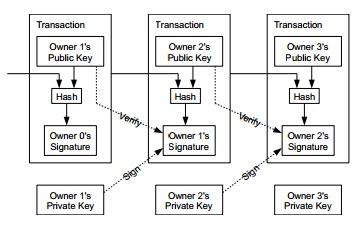
\includegraphics[width=.9\textwidth]{figures/transaction.png}
\end{figure}

\subsubsection{Transaction Blocks}
Once a transaction has been initiated it must be verified by users in the Bitcoin network in order for the transaction
to be fully committed. As transactions are sent out to the Bitcoin network, miners accumulate the transactions into a
block. As of January 2015, average size of each block varies greatly with a range of roughly 300 to 800 transactions per
block.\footnote{\url{http://blockchain.info/charts/n-transactions-per-block}} However, this size is increasing over time
as the average size ranged from roughly 200 to 400 only one year prior in January 2014. The size of these blocks ranges
from about 150KB to 450KB,\footnote{\url{http://blockchain.info/charts/avg-block-size}} creating a total size of 33GB
for the entire block chain.\footnote{\url{http://bitinfocharts.com/}}

\subsubsection{Verification Scheme}
Verification of a block requires some proof-of-work in order to complete the block and append it to the block chain. The
proof-of-work scheme used by the Bitcoin protocol is based on the Hashcash proof-of-work scheme proposed by Adam Back in
2002.~\cite{back02}. The original Hashcash specification was intended to prevent denial of service attacks in email
service but has found popular usage within the Bitcoin protocol.  To complete proof-of-work for a transaction, a SHA-256
hash with inputs of the previous hash and a nonce must be found such that the resulting hash is below a specified
difficulty level. In other words, we must feed the SHA-256 algorithm the previous hash of the coin concatenated with a
nonce or string such that we have a specified number of leading 0's in the resulting hash. One common way of computing
proof-of-work is using the following algorithm:
\vspace{1em}\\
\begin{algorithm}[H]
    \KwIn{$D$ = difficulty parameter, $P$ = previous transaction hash}
    \KwOut{$N$ = nonce, $H$ = resulting hash}
    $N \gets 0$\\
    $H \gets ${\sc SHA-256({\sc Concat($P, N$)})}\\
    \While{H $\ge$ D}{ $N \gets N + 1$\\
    $H \gets ${\sc SHA-256({\sc Concat($P, N$)})} }
    \Return{N, H}
\end{algorithm}
\vspace{1em}

Once a proof-of-work has been determined the block with the proof-of-work information is distributed to the Bitcoin
network. The difficulty of the proof-of-work operation is such that blocks are found for a transaction, globally on
average, in 10 minutes. This time is based on the global block difficulty which is determined by a ``moving average
targeting an average number of blocks per hour.''~\cite{nakamoto08} What this means is that periodically the speed at
which blocks are computed is evaluated and the global difficulty is adjusted accordingly\footnote{Difficulty evaluation
happens every 2016 blocks which is specified by the {\tt bitcoind} client at \url{http://github.com/bitcoin}}.

The node which distributes the completed block to the network is rewarded with bitcoins if the block is accepted. This
reward starts out at 50 bitcoins per block and is halved after every 210,000 blocks, which means that bitcoins
ultimately have an maximum quantity of roughly 21,000,000~\cite{nakamoto08}. Once Bitcoins are no longer awarded for
verifying blocks, the incentive must come from elsewhere. Fees can be attached to Bitcoin transactions, which simply
means that whoever verifies the block containing that transaction will receive the Bitcoins attached as a fee.

\subsubsection{Network Structure}
The original Bitcoin whitepaper~\cite{nakamoto08} describes the Bitcoin network in the following way: 
    \begin{enumerate}
        \item Transactions are broadcast to all network nodes.
        \item Transactions are collected and joined to form a block.
        \item A proof-of-work for a block is found, which is then broadcast to all nodes.
        \item If the proof-of-work is valid, all transactions in a block are valid, and bitcoins involved have not
            already been spent, then the block is accepted. 
        \item The accepted block is appended to the block chain, and its hash is now used as the input hash for the next
            block.
    \end{enumerate}

In other words, all nodes in the network are made aware of new transactions, verified transactions, and accepted blocks.
In this way the transaction record (block chain) is shared among all nodes in the network.

\subsection{Litecoin Protocol} Litecoin is the second most widely used cryptocurrency\footnote{\url{http://coinmarketcap.com} -- Accessed 3-18-14, Litecoin has the second highest 24 hour
trading volume}, and is itself a fork of Bitcoin. Litecoin's first block was mined in October
2011\footnote{http://ltc.blockr.io/block/info/1}. Litecoin has a few key differences from Bitcoin.  The primary
difference between Litecoin and Bitcoin is how the coins are mined, or rather how the transactions are verified. Rather
than using SHA-256 as a proof-of-work scheme Litecoin uses Colin Percival's scrypt~\cite{percival09}. Additionally,
rather than a global average of 10 minutes per block as in Bitcoin, Litecoin targets a global average of 2.5
minutes~\cite{sprankel13}. To prevent the reward pool of litecoins from drying up too quickly as a result of this faster
verification time, the number of blocks after which the reward is halved is quadruple that of Bitcoin. Rather than
halving after every 210,000 blocks, the reward for verifying a block halves after every 840,000 blocks.

\subsubsection{Transaction Scheme} The Litecoin transaction scheme is identical to that of Bitcoin. Litecoin also
records the signatures of all users involved, the amount being transferred in a block which is then itself part of a
larger block chain.

\subsubsection{Transaction Blocks}
Litecoin blocks are created the same way as Bitcoin. However, Litecoin's average block size is significantly smaller due
to its faster verification time and smaller trading volume. The monthly average number of transactions per Litecoin
block ranges from about 3 to 30.\footnote{\url{http://www.coindesk.com/data/litecoin-number-transactions-per-block/}}
Most blocks are smaller than 10KB, with the majority of blocks being on the order of several hundred bytes. The total
size for the Litecoin block chain is 3.95GB.\footnote{\url{https://bitinfocharts.com}}

\subsubsection{Verification Scheme}
Litecoin was forked from Bitcoin to address the strength that special purpose hardware brings to Bitcoin. Users in the
Bitcoin network with application specific integrated circuits (ASIC) designed specifically for computing SHA-256 hashes
have an enormous advantage over users without such hardware. To address this Litecoin uses the scrypt~\cite{percival09}
key derivation scheme instead of SHA-256, which changes the hashing scheme from a CPU-bound operation to a memory-bound
operation. By changing the verification problem from a CPU-hard to memory-hard problem, parallelization no longer
improves the speed of solving the problem. This yields the following Litecoin proof-of-work algorithm:
\begin{algorithm}
    \KwIn{$D$ = difficulty parameter, $P$ = previous transaction hash}
    \KwOut{$S$ = salt, $H$ = resulting hash}
    $S \gets 0$\\
    $H \gets ${\sc scrypt($P, S$)}\\
    \While{H $\ge$ D}{ $S \gets S + 1$\\
    $H \gets ${\sc scrypt($P, S$)}\\
    }
    \Return{S, H}
\end{algorithm}

\subsubsection{Network Structure}
The network structure of Litecoin, much like the transaction scheme, is virtually identical to that of Bitcoin. The
network nodes are users connected to the network who receive notifications of new transactions and verified
transactions.

\subsection{Economics}
Given that a bitcoin's value derives strictly from how much people are willing to pay for bitcoin, the value is quite
volatile. At Bitcoin's inception in 2009, BTC had no value whatsoever. Even four years later in January 2013 each BTC
was worth roughly \$13. However, during 2013 interest in Bitcoin skyrocketed which increased the value by 8000\% to a
staggering \$1100 per BTC.~\cite{ciaian2014economics} This Bitcoin craze eventually settled down and the price of BTC
has been slowly falling but tends to stay in the range of \$300 to \$500 per BTC.

Since the Bitcoin economy is so volatile it is very vulnerable to things such as inflation. In late 2014 about 50,000
of BTC were seized by the U.S. government and subsequently sold in an auction.\cite{reutersgov} The bitcoins ended up
being sold for a total of \$18.6 million, which was only slightly below the market value. Only one month later, the
price of BTC sits at around \$250. While it is difficult to draw direct relations between the two events, it is
certainly reasonable that the sudden sale of 50,000 BTC below market value would affect the market. While this is a
relatively small seizure of property, larger seizures and auctions could seriously affect the market. Additionally,
should a government entity have an opposition to Bitcoin, it would not be difficult to directly disrupt the market by
buying up BTC and deliberately selling at a significantly lower price. Alternatively, direct government statements can
dramatically impact BTC value. In December 2013, China declared that it does not recognize BTC as a legitimate currency
and that it has no value. This caused the value of BTC to rapidly decline to nearly half of its value within a few
weeks.\footnote{\url{http://www.cryptocoincharts.info/pair/btc/usd/btc-e/alltime}}

One of the largest economic concerns for BTC is tax evasion. Real-world cash transactions are taxed by the use of sales
tax. However, BTC can be spent freely without any taxation. Even if taxation is desired, it is difficult to figure out
which parties should be paying taxes (is this a purchase for a good, or perhaps just a birthday present to someone?),
what the tax rate should be (in which country or municipality is the purchase being made). With pure anonymity, none of
these questions can be answered with certainty. Some economists feel that in the future cryptocurrencies will become a
tax haven for wealthy individuals to hide their money and avoid paying taxes.\cite{marian2013}

An important observation to note is that these changes in BTC value also cause changes in the value of other
cryptocurrencies. The value of BTC and LTC tend to show the same change over time.\footnote{\url{http://www.cryptocoincharts.info/pair/btc/usd/okcoin/1-year}}~\footnote{\url{http://www.cryptocoincharts.info/pair/ltc/usd/okcoin/1-year}}
The implication of this is that drastic market changes in one cryptocurrency are likely to cause similar changes in
another market, which means that any given cryptocurrency has multiple attack vectors.

\section{Anonymity Characteristics}
\subsection{Current State of Cryptocurrency Anonymity}
Users in the Bitcoin community can be falsely led to the conclusion that their transactions are purely anonymous. For
example, WikiLeaks accepts bitcoin donations and states\footnote{\url{http://shop.wikileaks.org/donate} -- Accessed:
3-25-14},
\begin{quote}
    ``Bitcoin is a secure and anonymous digital currency. Bitcoins cannot be easily tracked back to you, and are safer
    and faster alternative to other donation methods.''
\end{quote}
This quote was published in 2011 yet still remains as stated on the WikiLeaks website as of January 2015 despite some
criticism of its accuracy.

Each transaction contains identifying information with respect to the addresses of the users. For every transaction in
the block chain, we can see between which users the transaction occurred as well as the number of bitcoins transferred.
Each of these transactions exists in the public transaction record to defend against double spending of bitcoins. Due to
the public nature of this record and the information associated with each transaction it is possible to deduce some, if
not all, information about users on the network.

One way to deduce information about users is based on the input addresses into a transaction. Since the private key
owning a bitcoin is required to initiate a transaction of that bitcoin, we can safely assume that in a transaction with
multiple input addresses that the addresses belong to one entity or person. The other possible scenario is that private
keys were shared, but this is an unlikely scenario. In fact, in the original Bitcoin whitepaper, Nakamoto
states~\cite{nakamoto08},
    \begin{quote}
        ``Some linking is still unavoidable with multi-input transactions, which
        necessarily reveal that their inputs were owned by the same owner.''
    \end{quote}

Much research has been done in this area already. In 2011, Reid and Harrigan analyzed one specific case of a theft of
25,000 BTC and attempted to trace the stolen BTC through the Bitcoin network~\cite{reid11}. One of the important results
from this study was that it was not extraordinarily difficult to follow the transfer of bitcoins between entities. The
authors were able to successfully trace the stolen bitcoins across many transfers and determine some specific addresses
to which the coins were transferred, such as LulzSec.

One way in which Nakamoto addresses this is suggesting that public keys be kept anonymous; however, this is not ideal or
even practical. Many users publish their public keys in forum signatures so that they may receive bitcoins.  In this
case, the public key is then very obviously associated with that specific username and passive analysis of multi-input
transactions can possibly reveal other keys associated with that user. Even if users do not publish their keys in this
way, some association may be revealed if a user takes advantage of services or stores that accept bitcoins. Consider the
case of a user wanting to exchange her bitcoins for some form of currency. To do so, she must go through some Bitcoin
exchange service, in which she necessarily reveals some personally identifying information to be able to receive her
money. She has now placed her anonymity in the hands of the exchange, since if the exchange is compromised her personal
information is also compromised.

In 2013 Ron and Shamir~\cite{ron13} performed analysis on the Bitcoin network using transaction size as their metric.
First they performed similar analysis to Reid and Harrigan to build a graph of entities, and then analyzed large
transactions to and from those entities. One of the first results from this analysis is that they were able to easily
identify a few key entities: Mt.  Gox\footnote{The largest bitcoin exhange at the time, filed for bankruptcy February
28, 2014}, Instawallet\footnote{Another large bitcoin exhange, shut down April 3rd, 2013.}, and DeepBit\footnote{The
largest mining pool at the time the study was performed.}.

Another key result determined from this analysis is the transaction patterns that are commonly used to attempt to
obscure a user's identity. The main activities identified by Ron and Shamir are long chains, fork-merge patterns, and
savings accounts. The long chains of transactions begin as one or more large transactions which are then split into many
smaller transactions in a very long chain. Fork-merge patterns are similar, except that the smaller transactions are
eventually merged back into one address. A large transaction gets split into multiple smaller transactions, but all
bitcoins ultimately end up back at the originating address. The last activity observed was the use of Bitcoin ``savings
accounts.'' Bitcoins are distributed across many addresses after which they are essentially untouched. A common pattern
for all of these activities is splitting a transaction into equal parts, which are then also split into equal parts,
etc. The resulting structure observed from this activity is akin to a tree~\cite{ron13}.

Researchers at University of California, San Diego and George Mason University~\cite{meiklejohn13} performed analysis on
change addresses in a Bitcoin transaction. They used the assumption that a one-time change address is controlled by the
same user as the input addresses. Based on this assumption, the authors were able to discover what they called ``peeling
chains,'' similar to activities observed by Ron and Shamir. This type of analysis was applied to a rather peculiar
Bitcoin wallet\footnote{Address: {\tt 1DkyBEKt5S2GDtv7aQw6rQepAvnsRyHoYM}}, in which an extremely large Bitcoin wallet
was split into several smaller wallets. These smaller wallets then eventually interacted with some Bitcoin services,
including exchanges. If this wallet were associated with an entity such as the Silk Road or the Bitcoin Savings \& Trust
Ponzi scheme~\cite{moore13}, the exchanges might be inclined to reveal identifying information about the user in
question, ultimately eliminating any notion of anonymity.

Using the result from these case studies we can clearly see that input addresses and change addresses can be used to
identify Bitcoin ``entities.'' We can also analyze these entities more closely and see how the entities try to obscure
their identity. Since these sorts of patterns are not extraordinarily difficult to deduce from the Bitcoin block chain,
one can imagine a scenario where some law enforcement agency might want to investigate a user who is a suspect in some
sort of illicit activity. We can determine a group of addresses that belong to the user, and if any of those addresses
interacted with a Bitcoin exchange or service, the law enforcement agency could seize the personal information of the
user from such a service. Even further, we can see all addresses with which the user interacted, which could implicate
other users involved in illicit activities. This allows the law enforcement agency to analyze these users more closely,
some of which may have interacted with a Bitcoin exchange, and so on.

\subsubsection{Initial Findings}
Based on our analysis of the cryptocurrency protocols and with the prior research that has been done in this area, we
can conclude that the base implementations of these cryptocurrencies do not offer the level of anonymity that is
typically advertised or desired by users. Since many users would eventually want to convert their bitcoins, litecoins,
or other coins into real-world currency, they will need to go through an exchange that requires personally identifiable
information. Alternatively, users could attempt to find someone willing to perform a cash exchange but this is far less
feasible.

Assuming that a person acquires some amount of bitcoins anonymously, spending the bitcoins anonymously can still be
difficult. Should a user want to spend their bitcoins at an actual business (since some businesses are now accepting
bitcoins as currency), they need to be sure that their information does not get leaked. If the user is making a purchase
online, then some form of information must be exchanged and then a possible attack vector is revealed. If the user makes
the purchase in an actual store, but then makes a purchase at a different store online, then there is still the same
risk of data leaking from the first store since all transactions are public. This can be solved by using a different
address for each store or transaction, but again this just falls back on Nakamoto's initial warnings that the only way
to remain truly anonymous is to do exactly that. This drastically reduces the usability of the systems, as this is
equivalent to using a different physical wallet for every cash transaction that a person makes, which is simply not
feasible.

The Bitcoin protocol was initially introduced to have a decentralized, anonymous, analog to real-world cash
transactions.  Users on a cryptocurrency network would ideally be able to conveniently exchange their coins without
having to give up their anonymity and privacy, while also not resorting to having a central authority. With the current
base implementations of these cryptocurrencies there is currently not support for maintaining pure anonymity without
expending extra effort to never reuse an address.

\subsection{Litecoin Transaction Graph}
In order to see if anonymity characteristics are present in other cryptocurrencies, we have performed analysis on the
Litecoin transaction ledger similar to what \mbox{Meiklejohn} et al.\ performed on the Bitcoin transaction
ledger\cite{meiklejohn13}. We parsed all Litecoin transactions to identify which addresses necessarily belong to the
same person. Our heuristic for this is if there are multiple addresses listed as input addresses in the same
transaction, they must belong to the same person. With this knowledge we can then build a graph of addresses with edges
between any addresses that belong to the same person. The end result is that each component in the graph represents an
entity within the Litecoin network.

\subsubsection{blockparser}
An important part of this analysis is the use of the open source \texttt{blockparser}\footnote{https://github.com/znort987/blockparser} tool. This tool provides a convenient way to view details (inputs,
outputs, total amount, etc.) of a given transaction. More specifically, we utilized a modified version that allows for
dumping all transaction metadata to .csv files for easier parsing\footnote{https://github.com/mcdee/blockparser}. We
used the output .csv files combined with some bash scripts to produce one single file that contains all transaction
hashes with multiple input addresses. We then used this single file to produce a file that contains all input addresses
used in these transactions grouped together by transaction.

\subsubsection{Algorithm}
The actual algorithm for identifying unique entities in the transaction graph is quite simple.
We represented each input address as a node in a graph, with two nodes being adjacent to each other if they are adjacent
in a list of input addresses to a single transaction. For example, suppose we have the following file:
\begin{verbatim}
A B C

D E

B F G

H I

E I
\end{verbatim}

From the contents of this file it can be seen that addresses \texttt{A}, \texttt{B}, and \texttt{C} were inputs to one
transaction and addresses \texttt{D} and \texttt{E} were inputs to another transaction. At a later point \texttt{B},
\texttt{F}, and \texttt{G} were inputs to a single transaction, which means that \texttt{A}, \texttt{B}, \texttt{C},
\texttt{F}, and \texttt{G} all belong to a single entity. When the transaction involving \texttt{H} and \texttt{I}
occurs, it cannot be tied to any previous entities. However, once the transaction with \texttt{E} and \texttt{I} occurs,
we can deduce that \texttt{D}, \texttt{E}, \texttt{H}, and \texttt{I} all belong to the same person. The result is the
following graph, where the nodes represent individual addresses and components represent entities.

\begin{center}
    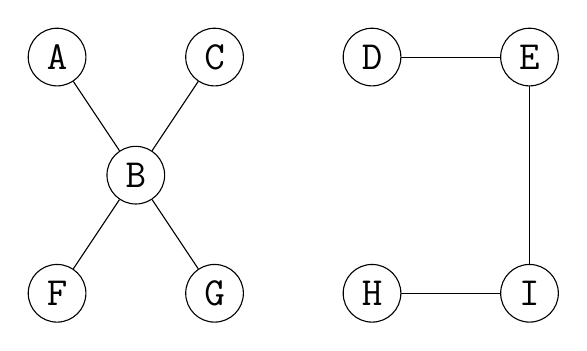
\begin{tikzpicture}[main node/.style={circle,draw,font=\ttfamily\Large\bfseries}]
        \node[main node] (1) at (0, 3) {A};
        \node[main node] (2) at (1, 1.5) {B};
        \node[main node] (3) at (2, 3) {C};
        \node[main node] (4) at (4, 3) {D};
        \node[main node] (5) at (6, 3) {E};
        \node[main node] (6) at (0, 0) {F};
        \node[main node] (7) at (2, 0) {G};
        \node[main node] (8) at (4, 0) {H};
        \node[main node] (9) at (6, 0) {I};
        \draw (1) -- (2) -- (3);
        \draw (6) -- (2) -- (7);
        \draw (4) -- (5) -- (9) -- (8);
    \end{tikzpicture}
\end{center}

Once this graph is constructed, performing a DFS on each component of the graph generates the following output:
\begin{verbatim}
Entity 1: A, B, C, F, G
Entity 2: D, E, I, H
\end{verbatim}

We implemented the algorithm using a number of Python and bash scripts. All code for the analysis can be found at:
    \begin{center} \texttt{http://github.com/lcm1115/Thesis/code/} \end{center}

\subsubsection{Results}
We ran our algorithm on all Litecoin transactions starting from block 0 on 10-07-2011 up through block 561763 on
05-05-2014. These blocks include 4,143,573 total transactions. The set of transactions \emph{T} which have multiple
inputs in a single transaction make up 901,424 of the transactions. Within \emph{T}, there are 1,718,624 distinct
addresses. After running the algorithm on the data set, we determined the following:
\begin{verbatim}
Number of distinct entities: 300,224
Average entity size (in # addresses): 8.76
Median group size: 2
Mode group size: 2
Largest group size: 1,030,616
\end{verbatim}

The total counts for each entity size can be found in the appendix.

With the largest group utilizing over half of the addresses used, we can draw similar conclusions to what Dorit and
Shamir determined in the Bitcoin transaction graph. That is to say, the entity to which these addresses belong is likely
a Litecoin exchange dealing with enormous volumes of transactions as well as personally identifying information about
users\cite{ron13}. If this is the case, then the same privacy risks exist within Litecoin as in Bitcoin, as any address
that has ever interacted with this large entity could have their privacy in this entity's hands.  Should the large
entity/exchange ever become compromised, then so does any user's data that was ever associated with it.

One thing worth noting is the comparison between the entity graph generated by the Litecoin transaction graph and
randomly generated graphs following the Erd\H{o}s-R\'{e}nyi model.\cite{erdos1959random} Given a $G(n, p)$ graph with
$n$ vertices and any edge having probability $p$, the graph has the following attributes:
\begin{itemize}
    \item If $np < 1$, then the size of any connected component is likely to be at most $O(log(n))$
    \item If $np = 1$, then there will likely be a large connected component whose size is $O(n^{2/3})$
    \item If $np > 1$, then there will likely be a unique giant component with a majority of the vertices, and there is
        unlikely to be any other component larger than $O(log(n))$.
    \item If $p < \frac{(1 - e) ln(n)}{n}$, then the graph is likely to be disconnected.
    \item If $p > \frac{(1 + e) ln(n)}{n}$, then the graph is likely to be connected.
\end{itemize}

Initially, the results of the experiment seemed to possibly reflect some of these properties. There certainly is one
unique giant component in the graph, and most components tend to be small. However, upon closer examination this is
about where the similarities end. With 4,143,572 transactions and an average of 2.57 inputs per transaction, this means
that there are approximately 10,648,980 edges in our entity graph. While this does not account for multi-edges,
multi-edges were rare enough that it should not significantly affect the number. With n = 1,718,624 distinct addresses
there are $\frac{n(n-1)}{2} = \frac{1,718,624(1,718,623)}{2} = 1,477,005,234,726$ possible edges in the graph. This
means that any given edge has probability $p = \frac{10,648,980}{1,477,005,234,726}$ of existing in the graph. We can
compute $np = 1,718,624 \cdot \frac{10,648,980}{1,477,005,234,726} = 12.39$. Indeed, this is the case in which there
should be a unique giant component with the majority of the vertices, and there is unlikely to be any component larger
than $O(log(n)) = O(log(1,718,624)) = O(6.24)$. However, this is absolutely not true of our graph, as there are several
hundred components much larger than this size.

\section{Improving Anonymity}
There have been many attempts to resolve the anonymity issues present in the Bitcoin protocol. Some of these attempts
have arisen organically within the Bitcoin community and are already in use, while others are proposed by academic
papers and have yet to be implemented.

\subsection{Mixer}
A very common form of obscuring one's identity is to use a mixer or tumbler\footnote{This name comes from the devices
used to clean physical coins.}.  These services are based on mix networks~\cite{chaum81}, which are used to mask a
user's identity within a network, such as the commonly used Tor network.  Unlike mix networks which are used to mix
messages and anonymize the users, Bitcoin mix services mix transactions to anonymize the users, frequently charging some
sort of processing fee for the service.

\begin{figure}[H]
    \caption[Example mix network]{Example mix network\protect\footnotemark}
    \centering
    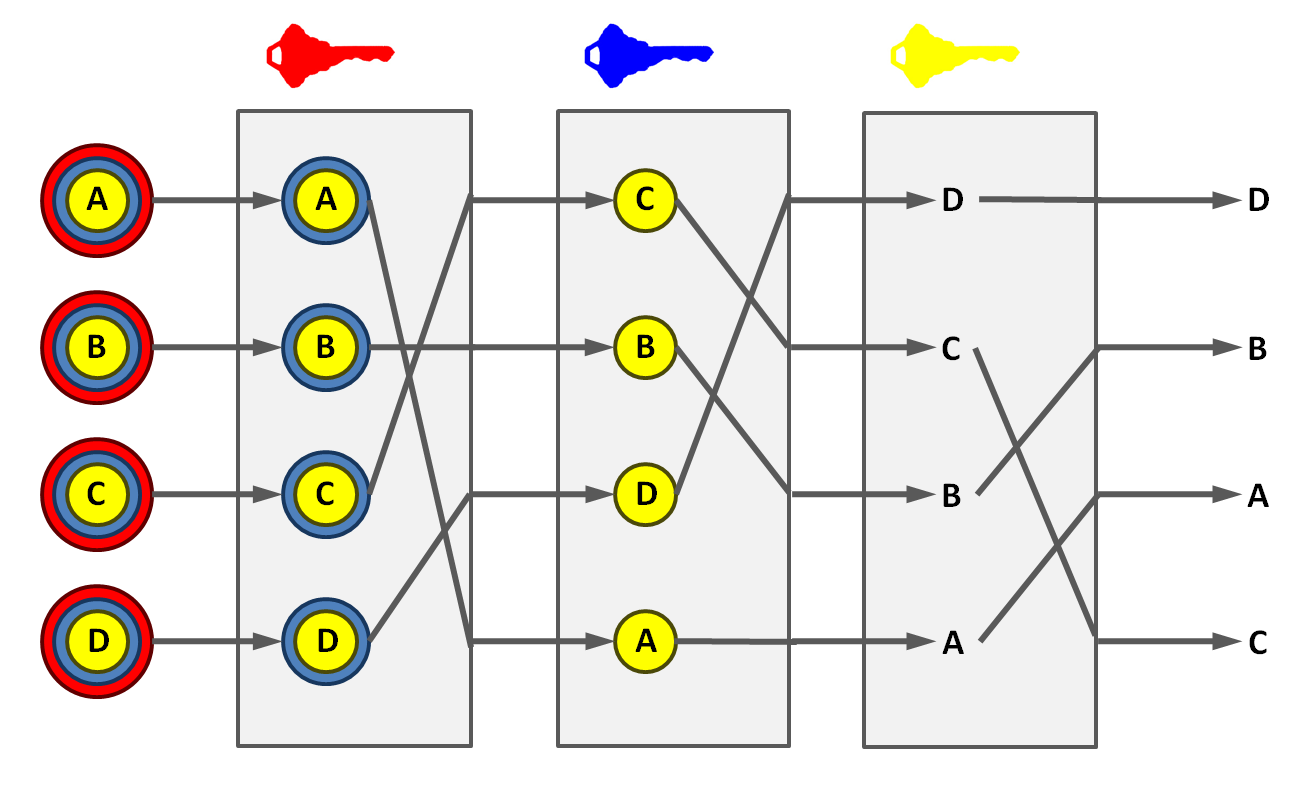
\includegraphics[width=.8\linewidth]{figures/mix.png}
\end{figure}

\footnotetext{\url{http://en.wikipedia.org/wiki/Mix_network} -- Accessed: 3-25-14}

A great deal of work has been done to analyze the anonymity provided by these services.  In 2013, Malte \Moser~analyzed
three popular mixing services: Blockchain.info, Bitcoin Fog, and BitLaundry~\cite{moser13}. The key results of this
experiment were that Blockchain.info and Bitcoin Fog both used complex methods of distributing transactions which
eliminate the ability to discover any connection between input and output transactions, effectively anonymizing the
traffic.  BitLaundry, on the other hand, used direction connections between input and output which allows for
connections to be drawn across the mixing operations.  This imperfect anonymization is present in other mixers. In
another study it was observed that Bitcoin Laundry took input transactions and directly fed them to output transactions
effectively eliminating the purpose of the service~\cite{meiklejohn13}. The possible cause for this is that the pool of
users in the service is to small to sufficiently anonymize transactions.

One of the primary issues in using these mixing or laundry services is that trust must be placed in the service which is
not an ideal scenario given that one of the goals of Bitcoin is to eliminate the requirement to place trust in
individuals. It has even been observed that these services cannot necessarily be trusted, as Meiklejohn reported that
``One of these, BitMix, simply stole our money.''~\cite{meiklejohn13} The presence of this behavior and the desire for
anonymity suggests that there is a desire for a system which provides anonymity without the need to place trust in some
sort of central figure.

\subsection{Zerocoin}
In 2013, researchers at Johns Hopkins University proposed an extension to improve Bitcoin's anonymity known as
Zerocoin~\cite{miers13}. The group claims that Zerocoin ``uses standard cryptographic assumptions and does not introduce
new trusted parties or otherwise change the security model of Bitcoin.'' The basic idea is to add newly minted coins to
an accumulator and then with the assistance of zero-knowledge proofs spend the coins from the accumulator without
revealing a user's identity.

The Zerocoin protocol essentially creates a currency within Bitcoin. To mint zerocoins, a user generates a random serial
number \emph{s} and a random nonce \emph{r}. These two values are then used as inputs to a Pedersen commitment to
receive resulting zerocoin \emph{C}. If \emph{C} is not prime, then a new \emph{r} is chosen until a prime value
\emph{C} is computed. Once the coin has been ``minted,'' it is sent to users to be added to the Zerocoin accumulator
which is based on the Strong RSA Accumulator. In order to spend these coins, a user sends out a transaction with the
coin serial \emph{C}, the values \emph{s} and \emph{r} that produce \emph{C}, and the address to which the coins should
be sent. Users verifying transactions can then confirm the presence of \emph{C} in the accumulator, while also verifying
that the values \emph{s} and \emph{r} are valid. Once this is confirmed the output address is then considered to be the
owner of the bitcoins associated with the zerocoin, and the accumulator must be recomputed with all values except
\emph{C}.

\begin{figure}[H]
    \centering
    \caption[Bitcoin block chain (a) and Zerocoin block chain (b)]{Bitcoin block chain (a) and Zerocoin block chain (b)~\cite{miers13}}
    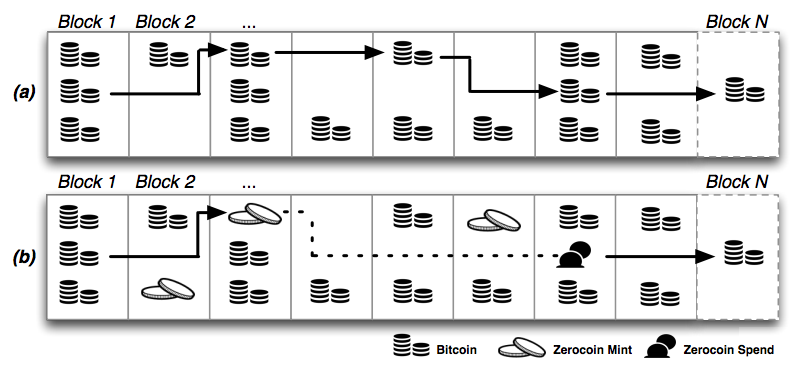
\includegraphics[width=\linewidth]{figures/zerocoin.png}
\end{figure}

This system creates anonymity since there is no way to link together the minting and spending operations of zerocoins.
Any user can spend any of the zerocoins as long as he can prove the existence of the zerocoin and the values associated
with its minting. In a sense, this is analogous to a mixing service, but there is no requirement to place trust in any
figure, as the system is provably secure under certain cryptographic assumptions. The only centralization in this system
is the establishment of the infrastructure used.

\subsubsection{Performance Concerns}
While Zerocoin appears to be a promising solution to the problem of anonymity on the Bitcoin network, performance is a
big concern. The use of 3,072-bit RSA accumulators is very computationally expensive, and every time a coin is spent
from the coin pool, the accumulator must be recomputed.

One of the big benefits to Zerocoin is that its simple nature allows it to be applied to any cryptocurrency that is a
derivation of Bitcoin. For cryptocurrencies with long block-verification times such as Bitcoin, the overhead from using
Zerocoin is fine. The Zerocoin whitepaper describes Zerocoin's performance, and even in a best case (for Zerocoin) and
worst case (for Bitcoin) scenario where blocks contain twice as many transactions than normal and every transaction is a
Zerocoin transaction, then the block verification process still takes five minutes.~\cite{miers13} Since Bitcoin has a
block verification time of ten minutes, this does not cause any problems as it does not affect the overall block
verification time.

If Zerocoin is utilized in Litecoin then problems may arise. If the same volume of transactions is seen in Litecoin,
then a five minute block verification time is unacceptable. Since Litecoin's block verification time is targeted at 2.5
minutes, adding Zerocoin effectively doubles the block verification time. Since this is the case, we wanted to determine
if there are methods of improving performance such that utilizing Zerocoin in other cryptocurrencies becomes
computationally feasible. The method we tried was substituting the 3,072-bit RSA accumulator for a 384-bit ECC
accumulator. Since 256-bit curves offer the same security as 3,072-bit integers, there is no loss of security or
privacy.\cite{nistcase}

Our method of testing was to use an RSA accumulator with a random 3,072-bit prime \emph{p} and accumulate a number of
3,072-bit random elements into it, with a corresponding ECC accumulator using Curve P-256~\cite{curves} into which a
random number of 256-bit elements are accumulated. The time for each accumulator is benchmarked, and results can be
found in the following table.
\begin{center}
\begin{tabular}{|c|c|c|c|}
    \hline
    \textbf{\# Elements} & \textbf{RSA Time (s)} & \textbf{ECC Time (s)} & \textbf{Performance Multiplier} \\
    \hline
    10,000 & 129.131 & 1.151 & 112.19 \\
    \hline
    20,000 & 257.768 & 2.3 & 112.073 \\
    \hline
    30,000 & 392.755 & 3.521 & 111.546 \\
    \hline
    40,000 & 527.18 & 4.571 & 115.331 \\
    \hline
    50,000 & 654.387 & 5.681 & 115.189 \\
    \hline
\end{tabular}
\end{center}

As is shown, using an ECC accumulator over an RSA accumulator offers massive performance gains. Assuming these gains
translate 1:1 to Zerocoin, the five minute Zerocoin verification time can be reduced to a few seconds. With such a quick
verification time, Zerocoin can now be used with Litecoin, and even cryptocurrencies with drastically shorter block
verification times such as Dogecoin, which has a one minute verification time. The end result overall is that there is
now an efficient and computationally feasible method of adding a layer of anonymity to most cryptocurrencies, provided
that the verfication time is on the order of minutes and not seconds.

\subsection{Mixcoin}
In 2014, another extension to improve anonymity in current Bitcoin protocol was proposed under the name of
Mixcoin~\cite{bonneau14}. This protocol describes a method of establishing mixing services with some concept of
warranty, rather than modifying the Bitcoin protocol itself.

In general, sufficiently large mixing services do an acceptable job at providing anonymity to users; however, these
services have an inherent risk in that users must entrust the service with their bitcoins in order to utilize the
service.  If a mixing service steals a user's bitcoins, there is no way to prove that the theft occurred. Mixcoin's goal
is to address this issue by proposing a construction for a mixing service that has built-in accountability.

The basic process behind Mixcoin is that before any mixing occurs, a user Alice contacts the mix service and declares
the following parameters~\cite{bonneau14}:\\
\begin{tabular}{cl}
    $v$ & the value (chunk size) to be mixed\\
    $t_1$ & the deadline by which Alice must send funds to the mix\\
    $t_2$ & the deadline by which the mix must return funds to Alice\\
    $\kappa_{out}$ & the address where Alice wishes to transfer her funds\\
    $\rho$ & the mixing fee rate Alice will pay\\
    $n$ & a nonce, used to pay randomized mixing fees\\
    $w$ & the number of blocks the mix requires to confirm Alice's payment
\end{tabular}
\vspace{1em}\\ 
Once the mix accepts the terms of the mix, a new escrow address $\kappa_{esc}$ is generated. All parameters plus
$\kappa_{esc}$ are returned to Alice, signed by the mixing service. This allows Alice to publicly claim with certainty
that the mixing service has stolen her funds in the event of theft, or in the case that the funds have not been
delivered to $\kappa_{out}$ by $t_2$.

As part of the Mixcoin protocol the authors suggest that a randomized mixing fee be paid to the service by the users.
The proposed method of randomized mixing fees is to establish some probability $\rho$ where the entire value may be
taken as a fee, and probability $(1 - \rho)$ that there is no fee at all. The means of randomly choosing the fee each
item is to be made publicly verifiable so that the mixer can be audited if necessary to ensure that it is not behaving
maliciously. The authors believe that by having this randomized mixing fee there is extra incentive to operate honestly
and thus provide a better, low-risk service to the users.

While Mixcoin resolves one of the issues with mixing services it does not solve every issue. The mixing service
still effectively behaves as a bank between users, which violates the goal of decentralized electronic cash.
Additionally, Mixcoin states that all records of a mix occurring should be deleted once the mix is completed. If
a mixer fails to do so and becomes compromised then the information of all users that have utilized the service
is also compromised.  Even though Mixcoin makes it easier for Alice to trust a mixer with her service, she still
needs to trust the service with her information. This means that even if Mixcoin is utilized that there still
may be some degree of traceability in the system.

\subsection{Stealth Addresses}
In 2014 a feature called \emph{stealth addresses} was added to a Bitcoin utility library called
\texttt{sx}.\footnote{\url{https://github.com/spesmilo/sx}} Stealth addresses are described as ``a powerful tool for
allowing one to accept Bitcoins using a public Bitcoin address while preventing passive observers from knowing your
transaction history.''\cite{stealth}

The cryptography supporting stealth addresses is based on the Elliptic Curve Diffie-Helman Key Exchange
Algorithm. In order to use a stealth address, Alice publishes a public key \emph{Q} which has a corresponding
private key \emph{d}. If Bob wants to pay Alice, he generates a new keypair with public key \emph{P} and private
key {e}. \emph{P} is then published in the transaction. Both parties can then compute a shared secret \emph{S}
where $S = dP = eQ$. Once this shared secret is established, a pay-to-address \emph{Q'} can be computed as $Q' =
Q + H(S)$ where \emph{H} is a hash function. Alice can then spend the transaction with private key \emph{d'}
computed as $d' = d + H(S)$.

The security present in stealth addresses depends on the security of ECDH. In this process the only information
publicly revealed is \emph{Q} and \emph{P}, so as long as the private keys \emph{d} and \emph{e} remain private
then Alice's identity remains private. Since Alice's identity is never revealed then this seems to be an ideal candidate
for preserving anonymity on the Bitcoin or similar networks. However, this process is equivalent to generating a new
address for every transaction, which Nakamoto even states is the only means of preserving pure
anonymity.\cite{nakamoto08} The only difference here is that the \emph{payer} generates the stealth address instead of
the \emph{payee}. This process still does not allow for a user to remain purely anonymous without needing to use a new
address for every transaction.

\section{Conclusion and Future Work}
\subsection{Conclusion}
Bitcoin was initially introduced to provide a direct digital equivalent to cash transactions. This means that any
transactions made on the Bitcoin network should be anonymous, convenient, and not require a central authority to sign
off on the transaction. Based on the research that we have performed, as well as the research aggregated from other
sources, we have determined that it is not possible to remain truly anonymous on the Bitcoin or Litecoin networks
without giving up either convenience or decentralization. 

The most promising method for maintaining anonymity is by being careful and never reusing an address for any purpose.
This drastically increases the amount of work required to perform a transaction and makes the protocol significantly
more inconvenient. As stated previously, this method of maintaining anonymity is equivalent to storing the cash received
from every real-world transaction in its own wallet or bank account, and only ever spending from one wallet or bank
account at a time. This clearly is not feasible in the real world, so using this method of maintaining privacy pushes
cryptocurrencies further from being equivalent to cash.

Other promising methods of maintaining anonymity involve using some sort of service. There exist mixer services which
allow users to launder their coins through a central store such that the inputs and outputs cannot be tied to each
other. These work well in theory, but this requires users to trust the service with their currency. In many cases, these
services were caught simply stealing users' currency. There are some proposals to improve these systems, such as
Mixcoin, but rather than preventing the initial problem they simply provide some proof that a problem occurred. However,
the biggest problem with these mixing services is that they violate the concept of decentralization present in
cryptocurrency protocols.

In our opinion the most likely method to succeed in improving anonymity is Zerocoin. Zerocoin utilizes distributed
accumulators in order to allow users to anonymously deposit and withdraw coins. This acts similarly to a mixer, but
since there is no central authority that must be trusted the system is more secure for the users. The main issue with
Zerocoin seems to be performance. We have analyzed these concerns and determined that the performance is quite slow in
the worst case, and would only get worse as the system gets more widely adopted and the cryptocurrency sees larger
trading volume. We addressed these concerns by proposing our own solution. Rather than using accumulators based on
3,072-bit RSA keys, we can use 256-bit ECC accumulators and get performance increases on the order of 100x speed
improvement.

As it stands right now, the base implementations of cryptocurrencies do not offer sufficient identity protection and
proposals to solve this problem fall flat. The potential solutions we have seen are either unusable, risky, insecure, or
computationally infeasible. As a result of all of this, we do not feel that true anonymity is something that can be
achieved within Bitcoin-based cryptocurrency protocols.

\subsection{Future Work}
In the future we would like to investigate the usage of SHA-3 as a hashing algorithm in cryptocurrencies. There are
already cryptocurrencies using SHA-3, such as MaxCoin\footnote{\url{http://www.maxcoin.co.uk/}} and Slothcoin, but these
are not nearly as widely used as Bitcoin or Litecoin. Since SHA-3 does not necessarily add any privacy or security
improvements over SHA-256, this investigation would be based purely on performance. However, it is worth researching
since sponge constructions are such recent developments and it is possible that some discoveries may be made which make
sponge constructions more desirable for anonymity.

Continued analysis on transaction graphs relative to random graph models is something worth exploring further. We
currently only compared our analysis of the entity graph to random models, but it is possible that the pure transaction
graph of one or more cryptocurrencies more closely relates to randomly generated graphs. If any correlation is found,
investigating how transaction volume affects similarity is another possibility.

Finally, we plan to analyze any new developments that are made in this area. With interest in cryptocurrencies and
maintaining of anonymity and privacy there will surely be new ideas and proposals made to make it easier to remain
anonymous on the cryptocurrency networks. There are new products being introduced frequently, such as
DarkWallet\footnote{\url{http://www.darkwallet.is/}}, which promise anonymity, ease of use, and security. We would like
to perform proper analysis and potentially audit any provided code to see if there is a risk of information leakage.

\bibliographystyle{acm}
\bibliography{references}

\newgeometry{left=1in,right=1in}
\section{Appendix}
\subsection{Source Code}
\lstinputlisting[language=Python]{code/inputs.py}
\lstinputlisting[language=Python]{code/groupHashes.py}
\lstinputlisting[language=bash]{code/getHashes.sh}
\lstinputlisting[language=C++]{code/bench.h}
\lstinputlisting[language=C++]{code/bench.cpp}

\subsection{Litecoin Component Sizes}
\begin{center}
\begin{supertabular}{|p{.2\textwidth}|p{.2\textwidth}|p{.2\textwidth}|p{.2\textwidth}|}
    \hline
    Entity Size & Number of Entities & Entity Size & Number of Entities \\
    \hline
    2 & 155767 & 3 & 62113 \\
    \hline
    4 & 30695 & 5 & 17663 \\
    \hline
    6 & 10360 & 7 & 5176 \\
    \hline
    8 & 3490 & 9 & 2521 \\
    \hline
    10 & 1121 & 11 & 918 \\
    \hline
    12 & 1269 & 13 & 979 \\
    \hline
    14 & 783 & 15 & 633 \\
    \hline
    16 & 491 & 17 & 478 \\
    \hline
    18 & 349 & 19 & 346 \\
    \hline
    20 & 434 & 21 & 433 \\
    \hline
    22 & 285 & 23 & 227 \\
    \hline
    24 & 315 & 25 & 170 \\
    \hline
    26 & 163 & 27 & 157 \\
    \hline
    28 & 139 & 29 & 111 \\
    \hline
    30 & 113 & 31 & 107 \\
    \hline
    32 & 93 & 33 & 89 \\
    \hline
    34 & 88 & 35 & 80 \\
    \hline
    36 & 79 & 37 & 59 \\
    \hline
    38 & 65 & 39 & 55 \\
    \hline
    40 & 72 & 41 & 63 \\
    \hline
    42 & 52 & 43 & 43 \\
    \hline
    44 & 39 & 45 & 49 \\
    \hline
    46 & 44 & 47 & 29 \\
    \hline
    48 & 28 & 49 & 35 \\
    \hline
    50 & 40 & 51 & 33 \\
    \hline
    52 & 24 & 53 & 30 \\
    \hline
    54 & 33 & 55 & 17 \\
    \hline
    56 & 20 & 57 & 21 \\
    \hline
    58 & 17 & 59 & 27 \\
    \hline
    60 & 35 & 61 & 17 \\
    \hline
    62 & 22 & 63 & 19 \\
    \hline
    64 & 22 & 65 & 16 \\
    \hline
    66 & 12 & 67 & 21 \\
    \hline
    68 & 15 & 69 & 16 \\
    \hline
    70 & 15 & 71 & 19 \\
    \hline
    72 & 6 & 73 & 13 \\
    \hline
    74 & 14 & 75 & 8 \\
    \hline
    76 & 12 & 77 & 12 \\
    \hline
    78 & 14 & 79 & 10 \\
    \hline
    80 & 23 & 81 & 17 \\
    \hline
    82 & 9 & 83 & 11 \\
    \hline
    84 & 12 & 85 & 12 \\
    \hline
    86 & 8 & 87 & 3 \\
    \hline
    88 & 8 & 89 & 9 \\
    \hline
    90 & 4 & 91 & 5 \\
    \hline
    92 & 7 & 93 & 7 \\
    \hline
    94 & 7 & 95 & 7 \\
    \hline
    96 & 8 & 97 & 5 \\
    \hline
    98 & 3 & 99 & 8 \\
    \hline
    100 & 6 & 101 & 8 \\
    \hline
    102 & 8 & 103 & 8 \\
    \hline
    104 & 6 & 105 & 8 \\
    \hline
    106 & 8 & 107 & 3 \\
    \hline
    108 & 8 & 109 & 7 \\
    \hline
    110 & 6 & 111 & 2 \\
    \hline
    112 & 7 & 113 & 1 \\
    \hline
    114 & 4 & 115 & 5 \\
    \hline
    116 & 4 & 117 & 1 \\
    \hline
    118 & 1 & 120 & 2 \\
    \hline
    121 & 5 & 122 & 3 \\
    \hline
    123 & 4 & 125 & 2 \\
    \hline
    126 & 7 & 127 & 9 \\
    \hline
    128 & 4 & 129 & 4 \\
    \hline
    130 & 2 & 131 & 3 \\
    \hline
    132 & 3 & 133 & 4 \\
    \hline
    134 & 2 & 136 & 7 \\
    \hline
    137 & 5 & 138 & 1 \\
    \hline
    139 & 4 & 140 & 3 \\
    \hline
    141 & 2 & 142 & 4 \\
    \hline
    143 & 4 & 144 & 5 \\
    \hline
    145 & 3 & 147 & 4 \\
    \hline
    149 & 1 & 150 & 5 \\
    \hline
    151 & 4 & 152 & 2 \\
    \hline
    153 & 3 & 154 & 3 \\
    \hline
    155 & 5 & 156 & 3 \\
    \hline
    157 & 3 & 158 & 1 \\
    \hline
    159 & 3 & 160 & 2 \\
    \hline
    161 & 2 & 162 & 3 \\
    \hline
    163 & 3 & 164 & 3 \\
    \hline
    166 & 2 & 168 & 1 \\
    \hline
    169 & 1 & 170 & 2 \\
    \hline
    171 & 3 & 172 & 4 \\
    \hline
    174 & 3 & 175 & 5 \\
    \hline
    176 & 3 & 180 & 3 \\
    \hline
    182 & 2 & 183 & 3 \\
    \hline
    184 & 1 & 185 & 2 \\
    \hline
    186 & 3 & 187 & 2 \\
    \hline
    190 & 1 & 191 & 4 \\
    \hline
    195 & 1 & 196 & 1 \\
    \hline
    197 & 1 & 198 & 2 \\
    \hline
    200 & 11 & 201 & 9 \\
    \hline
    203 & 4 & 204 & 1 \\
    \hline
    206 & 2 & 207 & 1 \\
    \hline
    208 & 1 & 209 & 1 \\
    \hline
    210 & 4 & 211 & 1 \\
    \hline
    212 & 2 & 213 & 1 \\
    \hline
    214 & 2 & 215 & 2 \\
    \hline
    216 & 2 & 217 & 1 \\
    \hline
    219 & 2 & 220 & 1 \\
    \hline
    221 & 1 & 222 & 3 \\
    \hline
    224 & 2 & 226 & 2 \\
    \hline
    227 & 1 & 229 & 1 \\
    \hline
    230 & 2 & 231 & 1 \\
    \hline
    232 & 2 & 234 & 1 \\
    \hline
    235 & 2 & 236 & 1 \\
    \hline
    238 & 3 & 239 & 3 \\
    \hline
    240 & 2 & 243 & 1 \\
    \hline
    244 & 1 & 248 & 1 \\
    \hline
    249 & 1 & 252 & 1 \\
    \hline
    254 & 1 & 256 & 1 \\
    \hline
    260 & 1 & 261 & 1 \\
    \hline
    262 & 1 & 266 & 1 \\
    \hline
    267 & 2 & 270 & 1 \\
    \hline
    271 & 2 & 272 & 1 \\
    \hline
    273 & 4 & 274 & 1 \\
    \hline
    275 & 2 & 276 & 1 \\
    \hline
    277 & 2 & 278 & 1 \\
    \hline
    282 & 1 & 284 & 2 \\
    \hline
    285 & 1 & 286 & 1 \\
    \hline
    287 & 1 & 288 & 1 \\
    \hline
    289 & 1 & 290 & 1 \\
    \hline
    291 & 1 & 294 & 1 \\
    \hline
    295 & 2 & 297 & 1 \\
    \hline
    299 & 1 & 302 & 1 \\
    \hline
    305 & 1 & 308 & 1 \\
    \hline
    309 & 1 & 311 & 1 \\
    \hline
    313 & 1 & 315 & 1 \\
    \hline
    318 & 1 & 319 & 3 \\
    \hline
    323 & 1 & 326 & 1 \\
    \hline
    327 & 1 & 329 & 1 \\
    \hline
    332 & 1 & 343 & 1 \\
    \hline
    345 & 1 & 347 & 1 \\
    \hline
    349 & 2 & 351 & 1 \\
    \hline
    352 & 1 & 355 & 1 \\
    \hline
    356 & 1 & 362 & 1 \\
    \hline
    364 & 2 & 366 & 1 \\
    \hline
    368 & 1 & 373 & 1 \\
    \hline
    376 & 1 & 377 & 2 \\
    \hline
    381 & 1 & 384 & 1 \\
    \hline
    385 & 1 & 389 & 1 \\
    \hline
    392 & 1 & 393 & 1 \\
    \hline
    394 & 1 & 399 & 2 \\
    \hline
    401 & 1 & 408 & 2 \\
    \hline
    416 & 1 & 418 & 1 \\
    \hline
    419 & 1 & 420 & 1 \\
    \hline
    423 & 1 & 425 & 1 \\
    \hline
    428 & 1 & 429 & 2 \\
    \hline
    434 & 1 & 435 & 1 \\
    \hline
    450 & 2 & 456 & 1 \\
    \hline
    457 & 1 & 459 & 1 \\
    \hline
    470 & 1 & 471 & 2 \\
    \hline
    473 & 2 & 474 & 1 \\
    \hline
    481 & 1 & 485 & 1 \\
    \hline
    486 & 1 & 487 & 1 \\
    \hline
    491 & 1 & 493 & 1 \\
    \hline
    495 & 1 & 496 & 1 \\
    \hline
    497 & 1 & 500 & 1 \\
    \hline
    505 & 1 & 509 & 1 \\
    \hline
    510 & 1 & 522 & 1 \\
    \hline
    534 & 1 & 540 & 1 \\
    \hline
    554 & 1 & 555 & 1 \\
    \hline
    558 & 1 & 561 & 1 \\
    \hline
    564 & 1 & 566 & 2 \\
    \hline
    585 & 1 & 589 & 1 \\
    \hline
    593 & 2 & 600 & 1 \\
    \hline
    611 & 1 & 614 & 1 \\
    \hline
    672 & 1 & 683 & 1 \\
    \hline
    687 & 1 & 690 & 1 \\
    \hline
    693 & 1 & 696 & 1 \\
    \hline
    698 & 1 & 708 & 1 \\
    \hline
    714 & 1 & 719 & 1 \\
    \hline
    729 & 1 & 734 & 1 \\
    \hline
    750 & 1 & 762 & 1 \\
    \hline
    778 & 1 & 799 & 1 \\
    \hline
    803 & 1 & 862 & 1 \\
    \hline
    882 & 1 & 901 & 1 \\
    \hline
    918 & 1 & 925 & 1 \\
    \hline
    942 & 1 & 955 & 1 \\
    \hline
    969 & 1 & 982 & 1 \\
    \hline
    994 & 1 & 998 & 1 \\
    \hline
    1007 & 1 & 1011 & 1 \\
    \hline
    1059 & 1 & 1076 & 1 \\
    \hline
    1140 & 1 & 1178 & 1 \\
    \hline
    1181 & 1 & 1208 & 1 \\
    \hline
    1212 & 1 & 1219 & 1 \\
    \hline
    1246 & 1 & 1251 & 1 \\
    \hline
    1253 & 1 & 1265 & 1 \\
    \hline
    1266 & 1 & 1275 & 1 \\
    \hline
    1299 & 1 & 1328 & 1 \\
    \hline
    1351 & 1 & 1431 & 1 \\
    \hline
    1477 & 1 & 1508 & 1 \\
    \hline
    1695 & 1 & 1729 & 1 \\
    \hline
    1760 & 1 & 1862 & 1 \\
    \hline
    1901 & 1 & 1906 & 1 \\
    \hline
    1938 & 1 & 2129 & 1 \\
    \hline
    2297 & 1 & 2482 & 1 \\
    \hline
    2508 & 1 & 2694 & 1 \\
    \hline
    2829 & 1 & 3110 & 1 \\
    \hline
    3199 & 1 & 3281 & 1 \\
    \hline
    3865 & 1 & 4350 & 1 \\
    \hline
    4353 & 1 & 4413 & 1 \\
    \hline
    4496 & 1 & 4920 & 1 \\
    \hline
    5002 & 1 & 5043 & 1 \\
    \hline
    5367 & 1 & 5748 & 1 \\
    \hline
    5886 & 1 & 8033 & 1 \\
    \hline
    8214 & 1 & 9042 & 1 \\
    \hline
    9659 & 1 & 10272 & 1 \\
    \hline
    12536 & 1 & 12871 & 1 \\
    \hline
    14797 & 1 & 15537 & 1 \\
    \hline
    16759 & 1 & 28815 & 1 \\
    \hline
    36298 & 1 & 53022 & 1 \\
    \hline
    1030616 & 1 & & \\
    \hline
\end{supertabular}
\end{center}

\end{document}
